\documentclass[12pt,journal]{IEEEtran}

\usepackage[utf8]{inputenc}
\usepackage{pgfplots}
\usepackage{caption}

\begin{document}

    \title{Derivative fundamentals}
    \author{Alejandro Salgado Gomez}

    \maketitle

    This article will try to explain as simple as posible the concept of a
    derivative. A derivatavie is the solution to one of the principal
    problems in calculus, which is how to calculate the tangent rect throught
    a point, in other words, how to calculate the rate of change of a function.

    This has a lot of practical applications in mathematics and the real
    world\\

    Lets start from the beginning, lets say we have two points that represent
    the state of something that is moving, the first one is the starting
    position and the second one is the final position. And we want to calculate
    how much is the change of the possition of this thing from the starting
    point to the final position. Here a ilustration

    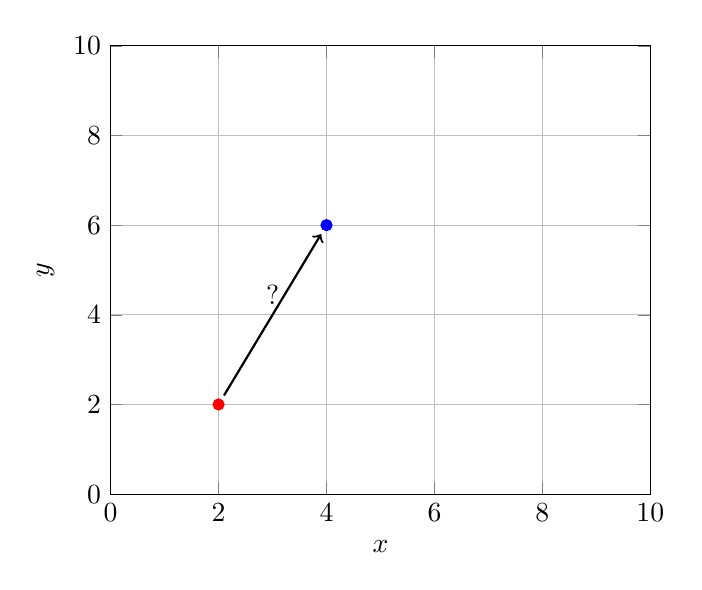
\begin{tikzpicture}
        \begin{axis}[
                      xlabel=$x$,
                      ylabel=$y$,
                      xmin=0, xmax=10,
                      ymin=0, ymax=10,
                      grid=both
                    ]
            \addplot[color=red, only marks]
                coordinates{
                    (2,2)
                };

            \addplot[color=blue, only marks]
                coordinates{
                    (4,6)
                };

            \draw[thick,->] (axis cs: 2.1,2.2) -- node[above]{?} (axis cs: 3.9,5.8);
        \end{axis}
    \end{tikzpicture}

    Notice that we are not interested in calculate the distance between this
    points, what we want is find a number that decribes how much the thing's
    position has change when he moves from the beginning to the end.

    This can be done by calculating for each unit of distance that the object
    has move, how much the object assend. This calculus can be  described as
    follows

    \begin{equation}
        change = \frac{ascend}{advance}
    \end{equation}

\end{document}
